\section{Theorie}
\label{sec:Theorie}

%\cite{sample}

\subsection{Schwingungsgleichung für kapazitiv gekoppelte Schwingkreise}
Betrachtet werden hier zwei gleiche elektrische Schwingkreise, die die Induktivität L und Kapazität C enthalten,
sie sind durch einen Kopplungswiderstand $ C_k$ gekoppelt.
Die Anwendung der Kirchhoffschen Knotenregel auf Punkt A liefer die Beziehung:
\begin{equation}
 I_k = I_1 - I_2
 \label{eqn:KK}
\end{equation}
Durch Anweung der Kirchhoffschen Maschenregel erhält man, für die Maschen 1 und 2, die Beziehungen:
\begin{equation}
  U_{1_{C}} + U_{1_{L}} + U_K = 0
  \label{eqn:KM1}
\end{equation}
 und
 \begin{equation}
   U_{2_{C}} + U_{2{L}} + U_K = 0
   \label{eqn:KM2}
 \end{equation}
 Mit den Beziehungen:
 \begin{equation*}
   U_C = \frac{1}{C} \int I_1 dt
 \end{equation*}
 und
 \begin{equation*}
   U_L = L\dot{I}
\end{equation*}
Durch die Verwendung dieser Beziehungen, Formel \eqref{eqn:KK} und Differentation nach der Zeit ergeben sich folgende Differentialgleichungen.
\begin{equation}
  L\ddot{I_1} + \frac{1}{C}I_1 + \frac{1}{C_k}(I_1 - I_2) = 0
  \label{eqn:Diff1}
\end{equation}
und
\begin{equation}
  L\ddot{I_2} + \frac{1}{C}I_2 + \frac{1}{C_k}(I_1 - I_2) = 0
  \label{eqn:Diff2}
\end{equation}
Nun wird die Summe und die Differenz der Einzelströme als Variablen eingeführt. Durch Subtraktion und Addition von \eqref{eqn:Diff1} und \eqref{eqn:Diff2} erhält man dann folgende Gleichungen.
\begin{equation}
  L \frac{d^2}{dt^2}(I_1 + I_2) + \frac{1}{C} (I_1 + I_2) = 0
  \label{eqn:Diff1p}
\end{equation}
und
\begin{equation}
  L \frac{d^2}{dt^2}(I_1 - I_2) + \left(\frac{1}{C} + \frac{2}{C_k}\right) (I_1 - I_2) = 0
  \label{eqn:Diff2m}
\end{equation}
Die Lösung von \eqref{eqn:Diff1p} ist die Gleichung einer harmonischen Schwingung.
\begin{equation}
  (I_1 + I_2)(t) = (I_{1_{0}} + I_{2_{0}}) cos \left(\frac{t}{\sqrt{LC}}\right)
  \label{eqn:diffi+i}
\end{equation}
Die Schwingungsfrequenz
\begin{equation}
  \nu_+ = \frac{1}{2\pi\sqrt{LC}}
  \label{eqn:nu+}
\end{equation}
ist gleich der eines Einzeloszillators. Daraus ist ersichtlich, dass die Amplitude mit $ I_{1_{0}} + I_{2_{0}} $ gegeben ist. Entsprechendes gilt für die
Differentialgleichung \eqref{eqn:Diff2m}.
\begin{equation}
  (I_1 - I_2)(t) = (I_{1_{0}} - I_{2_{0}}) cos \left(\frac{t}{\left(L\left(\frac{1}{C} + \frac{2}{C_k}\right)^{-1}\right)^{\frac{1}{2}}}\right)
  \label{eqn:diffi-i}
\end{equation}
Hier ist die Frequenz:
\begin{equation}
  \nu_- = \frac{1}{2\pi \left(L\left(\frac{1}{C} + \frac{2}{C_k}\right)^{-1}\right)^{\frac{1}{2}}}
\label{eqn:nu-}
\end{equation}
Durch Addition und Subtraktion von den Differentialgleichungen \eqref{eqn:diffi+i} und \eqref{eqn:diffi-i} erhält man für die Variablen $I_1$ und $I_2$ folgende Gleichungen.
\begin{equation}
  I_1 (t) = \frac{1}{2}(I_{1_{0}} + I_{2_{0}}) cos(2 \pi \nu_+ t) + \frac{1}{2}(I_{1_{0}} - I_{2_{0}})cos(2 \pi \nu_- t)
  \label{eqn:diffi1t}
\end{equation}
und
\begin{equation}
  I_2 (t) = \frac{1}{2}(I_{1_{0}} + I_{2_{0}}) cos(2 \pi \nu_+ t) - \frac{1}{2}(I_{1_{0}} - I_{2_{0}})cos(2 \pi \nu_- t)
\label{eqn:diffi2t}
\end{equation}
Nun können drei Fälle betrachtet werden.
\begin{enumerate}
  \item Beide Schwingkreise haben die selbe Phase und Amplitude. Also gilt $I_{1_{0}}= I_{2_{0}}$, dann schwingen beide Schwingkreise mit der Frequent $\nu_+$.
  Die Ströme $I_1$ und $I_2$ kompensieren sich also ständig, folglich liegt am Koppelkondensator $C_k$ nie eine Spannung an.
  \item Die Schwingkreise haben wieder die selbe Amplitude aber sind gegenphasig ($I_{1_{0}}= - I_{2_{0}}$). Nun schwingen beide Schwinkreise gegenphasig mit der Frequenz $\nu_-$.
   Diese Fälle werden als Fundermentalschwingungen bezeichnet.
  \item Nun soll Schwingkreis 1 eine Amplitude ungeleich Null haben und sich der Schwingkreis 2 in Ruhe befinden zum Zeitpunkt $t= 0$ ($I_{1_{0}}\neq 0 , I_{2_{0}}= 0$).
  Dann folgt aus den Gleichungen \eqref{eqn:diffi1t} und \eqref{eqn:diffi2t}:
\end{enumerate}
  \begin{equation}
    I_1 (t) = I_{1_0} cos \left( \frac{(\omega_+ + \omega_-)t}{2}\right) cos \left( \frac{(\omega_+ - \omega_-)t}{2}\right)
  \label{eqn:dcos}
  \end{equation}
  \begin{equation}
    I_2 (t) = I_{1_0} sin \left( \frac{(\omega_+ + \omega_-)t}{2}\right) sin \left( \frac{(\omega_+ - \omega_-)t}{2}\right)
  \label{eqn:dsin}
  \end{equation}
  Angenommen die Frequenzen $ \nu_+$ und $ \nu_-$ wären fast gleich , also $ C_k >> C $ , dann gilt:
  \begin{align}
    \frac{\left(\omega_+ + \omega_- \right)}{2} \approx \omega_+ \\
     \omega_- - \omega_+  << \omega_+
  \end{align}
  Aus den Gleichungen \eqref{eqn:dsin} und \eqref{eqn:dcos} ist ersichtlich, dass die Schwingkreise mit der Frequenz $\frac{(\nu_+ + \nu_-)}{2}$ schwingen. Die Amplitude ändert sich
  dabei periodisch mit der Frequenz $ \nu_- - \nu_+$ und nimmt dabei Werte von Null bis $ I_{1_0}$ an. Diese Schwingung wird Schwebung genannt. Hier schwingt die Energie periodisch zwischen
  den jeweiligen Schwingkreisen. Die Periode $T^*$ ist dabei duch folgendne Zusammenhang gegeben.
  \begin{equation}
      \frac{(\omega_- - \omega_+)T^*}{2} = \frac{\pi}{2}
  \end{equation}



  \subsection{Berechnung des Stromes in einem Schwingkreis in Abhänigkeit von der Frequenz}
  Im Folgendem werden Schwingkreise betrachtet, die durch eine Sinusspannung zum schwingen angeregt werden. Alle Berechnungen werden am Beispiel der Schaltung \ref{fig:Abb4} gezeigt.
  Sämtliche Verluste werden durch ohmische Wiederstände R dargestellt.
  \begin{figure}
    \centering
    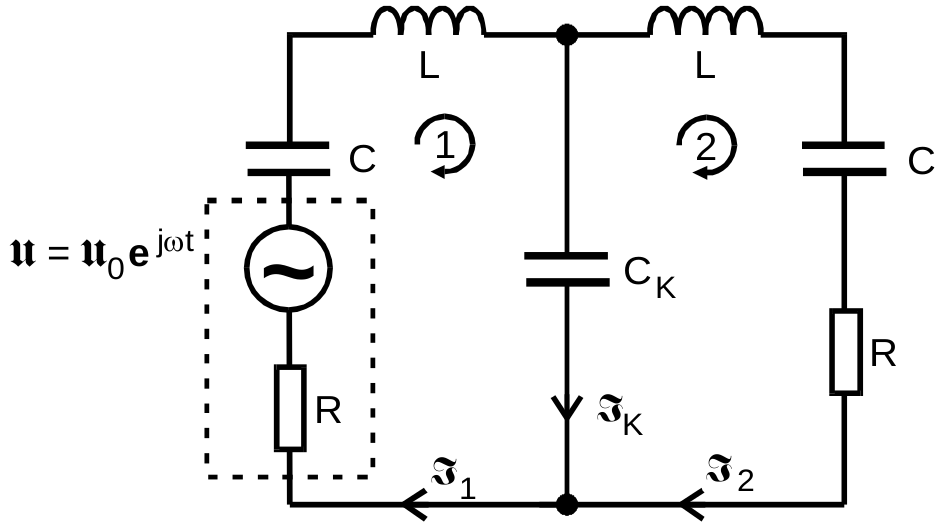
\includegraphics[width=\textwidth]{./logos/Abb4.png}
    \caption{Gekoppelte Schwinkreise mit eingebautem Sinusgenerator}
    \label{fig:Abb4}
  \end{figure}
  Dann folgt nach Kirchhofscher Maschenregel  für den Kreis
  \begin{enumerate}
    \item
    \begin{equation}
        (z_C + z_L + z_{C_R} + z_R)I_1 - z_{C_K} I_2 = U
        \label{eqn:U1}
    \end{equation}
    \text{und}
      \item
      \begin{equation}
          (z_C + z_L + z_{C_R} + z_R)I_2 - z_{C_K} I_1 = 0
          \label{eqn:U2}
      \end{equation}

  \end{enumerate}
  mit
  \begin{align*}
    z_C & =  -i \frac{1}{\omega C} & z_L & =  i\omega L \\
    z_{C_K} & = -i \frac{1}{\omega C_K} &  z_C & =  R
  \end{align*}
Aus diesen Beziehungen erhält man dann für den Betrag von $I_2$:
\begin{equation}
  \lvert I_2 \rvert = \lvert U \rvert \frac{1}{\left( 4\omega^2 C_{K}^2 R^2 Z(\omega)^2 + \left( \frac{1}{\omega C_K}-\omega C_K Z(\omega)^2 + \omega R^2 C_K\right)^2 \right)^{\frac{1}{2}}}
  \eqcolon \lvert U \rvert \cdot \lvert \symfrak{L} \rvert
  \label{eqn:UL}
\end{equation}
\text{mit}
\begin{equation*}
Z(\omega) \coloneq  \omega L - \frac{1}{\omega}\left(\frac{1}{C} + \frac{1}{C_K} \right)
\end{equation*}
Duch Gleichung \eqref{eqn:UL} ist ersichtlich, dass für $\omega$ gegen Null, sowie gegen Unendlich gegen Null geht. Dazwischen liegen die Fundermentalfrequenzen \omega_{\pm} für
die $\lvert \symfrak{l} \rvert $ ein Maximum durchläuft.
